
\begin{figure*}[ht!]
\centering
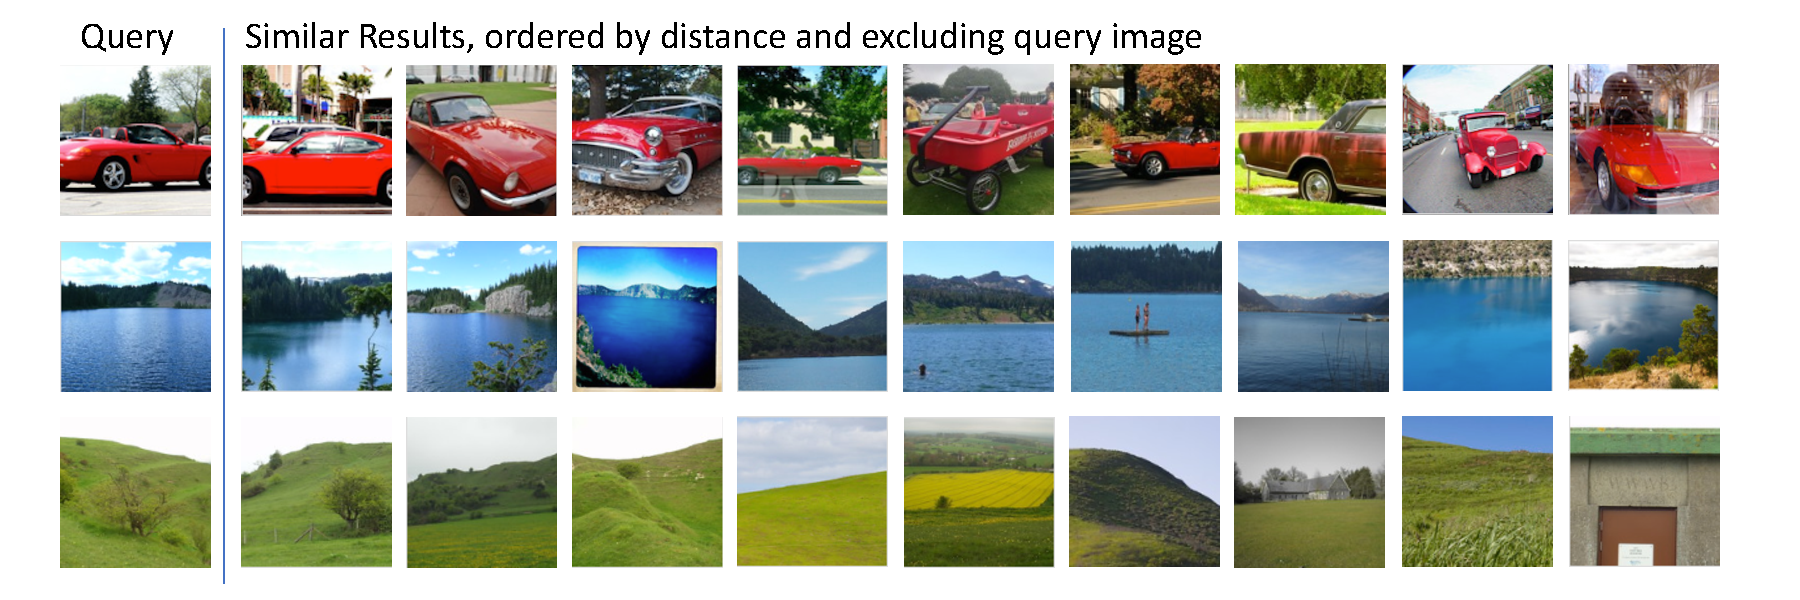
\includegraphics[width=\textwidth]{figures/feature_img_results}
\caption{Sample Results of Similarity Search}
\label{fig:similarity}
\end{figure*}

\subsection{Similarity Search}
\label{features}

Another key differentiating factor of VDMS is that it allows the creation of
indexes for high-dimensional feature vectors and the insertion of
these feature vectors associated with entities, images, and/or videos.
Feature vectors are intermediate results of various machine
learning or computer vision algorithms when run on visual data.
Feature vectors are also known as \textit{descriptors}
or \textit{visual descriptors}. We use these terms interchangeably.
These descriptors can be classified, labeled, and used to build search
indexes. There are many in-memory libraries that are designed for
this task~\cite{flann, faiss}.

% We analyze the behavior of the feature vector functionality in VDMS,
% and an evaluation of the different trade-offs that the systems offers for
% application developers. For this, we implemented an image-search application
% based on \textit{similarity} search.

Using the VDMS API, users can manage feature vector indexes,
query previously inserted elements,
run a k-nearest neighbor search (\textit{knn}), and express relationships
between existing images or descriptors and
the newly inserted descriptors.
By natively supporting descriptors and \textit{knn},
VDMS allows out-of-the-box classification functionalities for many applications
\footnote{https://github.com/\{Not shown during submission\}}.
% \footnote{https://github.com/IntelLabs/vdms/wiki/ClassifyDescriptor}.

For this work, and as part of a comprehensive image search implementation,
we have used 4096-dimensional descriptors extracted from every image
(and first frame of every video) from the YFCC100M dataset
and created a collection of these feature vectors in VDMS to
perform similarity search (i.e., find images that are
\textit{similar} to an query (input) image).
\textit{Similarity} in this particular case is defined as closeness
in a 4096-dimensional space using euclidean distance as the metric.

The process of loading descriptors in VDMS is simple.
First, the user has to create a DescriptorSet, using a single command.
At creation of the DescriptorSet, the dimensionality of the descriptors
is specified, together with the desired indexing method and the desired metric
for computing distances (Euclidean Distance, \textit{L2},
or Inner Product, \textit{IP}).
Once the DescriptorSet is created, descriptors can be inserted to the set.
After the descriptors are inserted, a similarity search can be performed.

Figure~\ref{fig:similarity} shows 3 examples of a query image (on the left),
and images returned as \textit{similar} by VDMS.
The input is a descriptor generated after a query image.
The \textit{query input} descriptor is sent to VDMS as part of the query,
VDMS uses that descriptor to find similar ones,
and retrieves the images associated with those \textit{similar} descriptors.
We show this as an example of the functionality and to depict
how the feature vectors provided by the dataset can be used,
but we also provide an analytical approach to
the trade-off between accuracy and execution time in our system.
It is important to note that the accuracy of the results is entirely tied
to the quality of the descriptors chosen by the applications.
The quality of the similarity result will be tied to the quality
of the descriptor extraction that the application is using.

\begin{figure*}[ht]
\centering
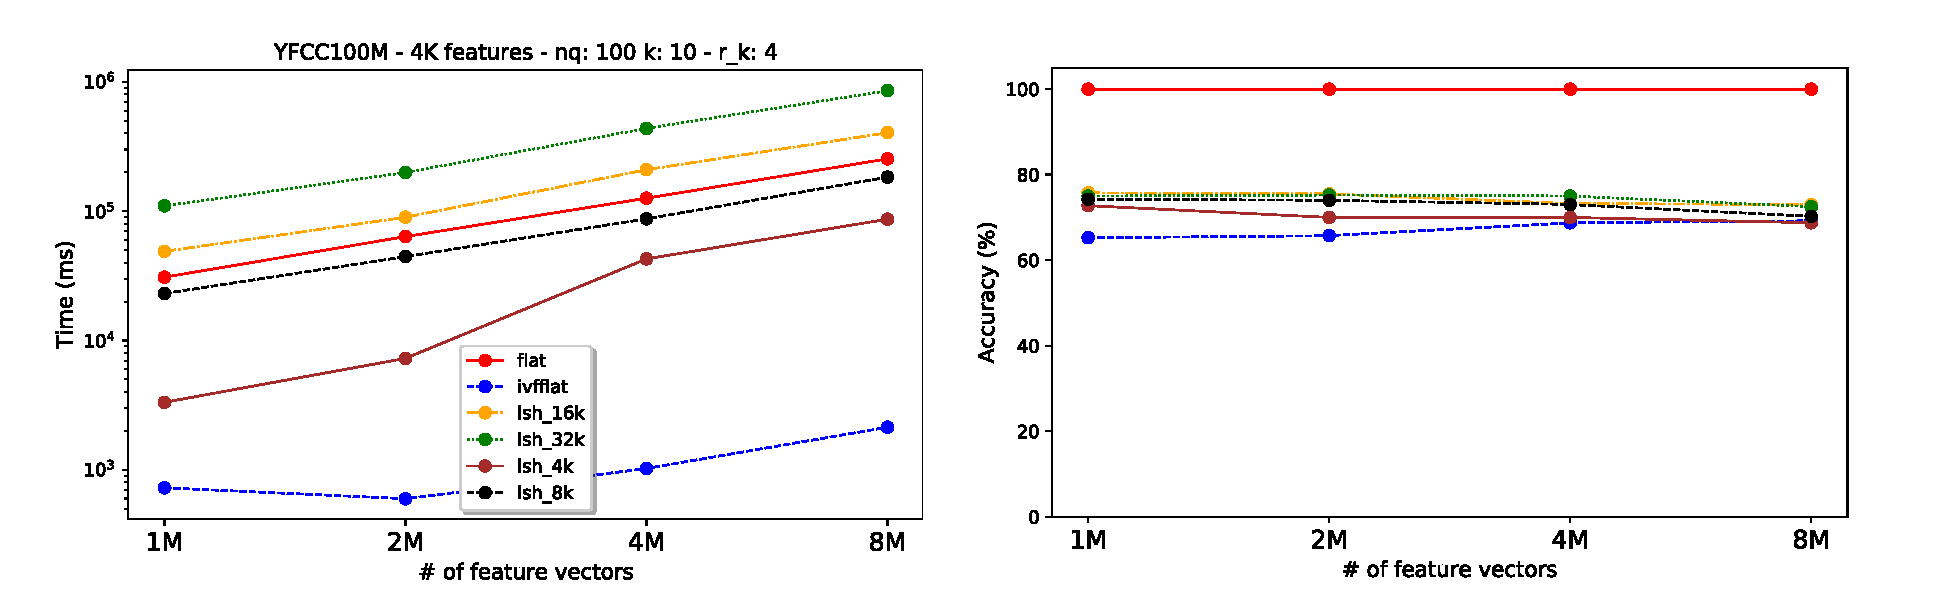
\includegraphics[width=\textwidth]{figures/features_alternatives}
\caption{Feature Vector Evaluation: Trade-off between query execution speed
and accuracy of the results, using ground-truth data for computing accuracy.
For this evaluation, we query the 10 closest neighbors (k = 10), and compute
accuracy using recall at 4 (r\_k = 4) (i.e. percentage of the top 4 ground-truth
results that is present within the top 10 computed neighbors).
We average the query execution time and accuracy for 100 queries (nq = 100).}
\label{fig:features_eval}
\end{figure*}

\begin{figure*}[ht]
\centering
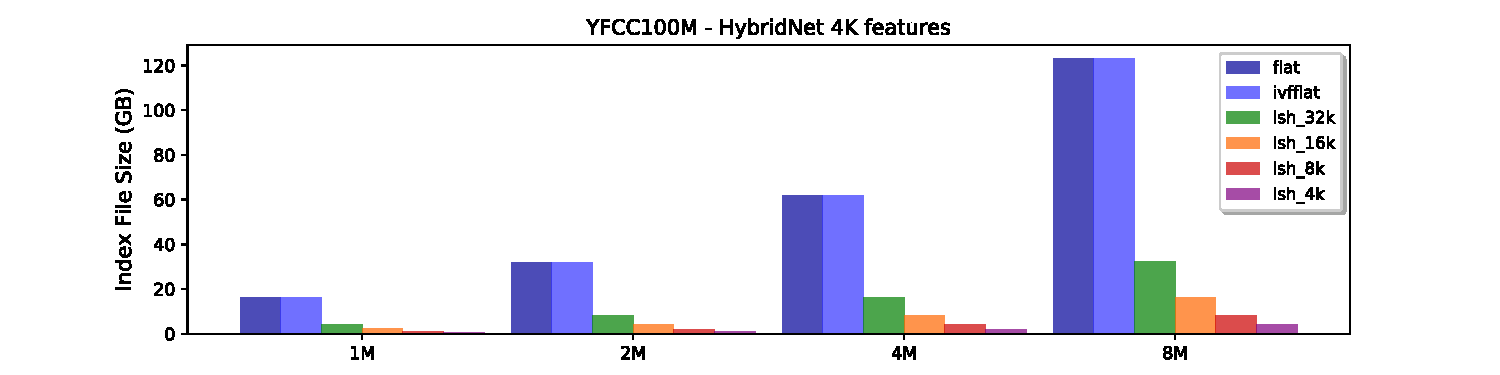
\includegraphics[width=\textwidth]{figures/features_disksize}
\caption{Feature Collection Size in Disk}
\label{fig:features_size_does_matter}
\end{figure*}

As mentioned before, VDMS provides different levels of customization of the
indexes created for a descriptor set, that includes the indexing techniques
and the metric for similarity.
These different indexing techniques come with different trade-offs in terms
of speed of search and accuracy of the computation.
VDMS aims to provide functionality that is agnostics to application-specific
techniques, enabling features that are generic to visual data processing
applications.
Figure~\ref{fig:features_eval} shows an analysis at the different indexing
techniques provided by VDMS and its trades-off between accuracy and query
execution speed, for a single threaded client.
For this evaluation, we query the 10 closest neighbors (k = 10), and compute
accuracy using recall at 4 (r\_k = 4) (i.e. percentage of the top 4 ground-truth
results that is present within the top 10 computed neighbors).
We average the query execution time and accuracy for 100 queries (nq = 100).
The \textit{flat} index (red line) implements exact search and
represents ground-truth, which explain why the
accuracy is always 100\% in the plot on the right.
The other indexes implement \textit{approximate search},
which trades-off between accuracy and speed of search~\cite{flann, faiss}.
We have also tried the \textit{ivfflat} index (inverted file index), as well as
\textit{LSH}-based indexes using a different number of bits per descriptor
\footnote{https://github.com/facebookresearch/faiss/wiki/Faiss-indexes}.
Results show how \textit{ivfflat} is the fastest option but it comes with a trade-off
of about 30\% loss in accuracy, while simple brute-force search
is among the slowest options at the expenses of 100\% accuracy,
meaning exact search.

Another important trade-off to be made is with respect to space efficiency:
The DescriptorSet can grow very large and expensive to load and manage.
In this particular case, 4096-dimensional descriptors for 100M elements
translates into 1TB of data, only in raw floating-point data alone
(without accounting for any metadata or indexes associated with it).
This component is very important for the overall analysis on which
index structure to use because a large set of descriptors may not fit in memory
and thus cause a pressure on the IO system while retrieving descriptors
for computing distance.
This can severely impact the overall query execution time.
When the DescriptorSet grows significantly large,
it may be worth trading off accuracy for speed and space.
Figure~\ref{fig:features_size_does_matter} shows the different indexes and
their size in disk. These indexes already contain all the descriptors (or
a quantized version of them in the case of LSH~\cite{lsh}),
and can be loaded in memory directly when it fits.
Note how, because of quantization of the descriptors, \textit{LSH} provides a
significantly lower space foot print, which can be a great option for
large collections of descriptors when accuracy is not a main factor.
It is not uncommon to sacrifice accuracy as images and videos are captured
using a noise sensor (i.e., the camera), and an approximate search
in many cases can provide the necessary accuracy for applications
to achieve their goals.
